\documentclass[12pt, t]{beamer}
\usepackage{amsmath}
\usepackage{setspace}
\usepackage{float} 
\usepackage{multido}
\usepackage{multirow}
\usepackage{array}
\usepackage{enumerate}
\usepackage{booktabs}
\usepackage{indentfirst} 
\usepackage[style=mla]{biblatex}
\usepackage{setspace}
\usepackage{subcaption}
\usepackage{hyperref}
\usepackage{textpos}

\makeatletter
\let\@@magyar@captionfix\relax
\makeatother

\definecolor{Turquoise3}{RGB}{0, 134, 139}
\renewcommand{\emph}[1]{{\color{Turquoise3}\textsl{#1}}}
\newcommand{\C}{\mathbb{C}} \newcommand{\F}{\mathbb{F}} \newcommand{\R}{\mathbb{R}} \newcommand{\Q}{\mathbb{Q}}
\newcommand{\N}{\mathbb{N}}
\newcommand{\myseries}[2]{$#1_1,#1_2,\dots,#1_#2$}
\newcommand{\nullspace}{~\\[15pt]}
\newcommand{\Remark}{\textbf{Remark: }}
\newcommand{\Question}{\textbf{Question: }}
\newcommand{\Extension}{\textbf{Extension: }}
\newcommand{\scp}[2]{\langle\,#1\,,\,#2\,\rangle} \newcommand{\scpp}{\langle\,\cdot\,,\,\cdot\,\rangle}


\usetheme{Madrid}
\setbeamertemplate{navigation symbols}{}

\addtobeamertemplate{frametitle}{}{
\begin{textblock*}{100mm}(0.85\textwidth,-1cm)

\includegraphics[height=1cm]{logo.png}
\end{textblock*}}

\definecolor{themecolor}{RGB}{25,25,112} 

\usecolortheme[named=themecolor]{structure}

\setbeamertemplate{items}[default]

\hypersetup{
    colorlinks=true,
    linkcolor=themecolor,
    filecolor=themecolor,      
    urlcolor=themecolor,
    citecolor=themecolor,
}

\title{VV285 RC Part VII}
\subtitle{\textbf{Differential Calculus}\\\large Integral in $\R^n$}
\institute[UM-SJTU JI]{Univerity of Michigan-Shanghai Jiao Tong University Joint Institute}
\author{Xingjian Zhang}

\begin{document}

\begin{frame}
    \titlepage
    \begin{center}
        
\includegraphics[height=2cm]{logo2.png}
    \end{center}
\end{frame}

\section{Integral in Multidimensional Vector Space}
\begin{frame}
    \frametitle{Outline}
    \begin{spacing}{1.2}
        \tableofcontents[currentsubsection,hideothersubsections,sectionstyle=hide]
    \end{spacing}
\end{frame}

\begin{frame}
    \frametitle{Something you need to pay attention to...}
    Think More and Be Interactive!
    \begin{itemize}
        \item Do think more about the question in ``()''. \\e.g. ``(How to prove?)''
        \item You are welcome to ask questions in a adequate manner.
        \item Please open your camera so that I can receive more feedbacks from you. (Makes our life easier!)
        \item The class is designed to be interactive. However, if you really do not want to be asked at all, please type an ``\_'' before your zoom name.
    \end{itemize}
\end{frame}

\subsection{Overview}
\begin{frame}[allowframebreaks]
    \frametitle{Overview}
    At this moment, we have learned how to perform integral in finite dimensional vector space. To be more specific, we have investigated deeply into the volume and (hyper-)surface integral in $\R^n$. Additionally, powerful integral tools such as Fubini's theorem and substitution rule were introduced. Therefore, you are supposed to be able to figure out many complex integrals in high-dimensional space on your own! For example, the surface area and volume of a \emph{hyperball} in $\R^5$. And that's something you will not be surprised if encountered during exams. In lectures, for most of time, we limited ourselves in $\R^2$ and $\R^3$. Thus, you should be particularly experienced to perform integral in both space.
    \newpage
    Trust me, you will reopen your VV285 lecture slides again and again in your future study, no matter what your major is! (Hopefully, some of you will reopen my RC slides) Here is a list of courses where you will find learning well in VV285 is so useful:
    \begin{enumerate}
        \item VV214 \& 417: Linear Algebra
        \item VV286: Honors Math IV
        \item VV556 \& 557: Methods of Applied Mathematics I\&II
        \item VP150/160 \& VP250/260: (Honors) Physics I\&II
        \item VP390: Modern Physics
        \item VE230 \& VE330: Electromagnetics I\&II
        \item VM211: Introduction to Solid Mechanics
        \item VM320 \& 520: Fluid Mechanics \& Advanced Fluid Mechanics
        \item \dots
    \end{enumerate}
    \newpage
    In summary, you need to be particularly experienced to perform any integral in $\R^2 \& \R^3$.{i.e. Line integral/surface integral/volume integral on scalar/vector function, we haven't introduced some of which.}
\end{frame}

\subsection{Cuboids}
\begin{frame}
    \frametitle{Cuboids}
    Let $a_k,b_k,k=1,\ldots,n$ be pairs of numbers with $a_k<b_k$. Then the set $Q\subset\R^n$ given by
    \begin{equation*}
        \begin{split}
            Q &=[a_1,b_1]\times\cdots\times[a_n,b_n] \\
            &=\{x\in\R^n:x_k\in[a_k,b_k],k=1,\ldots,n\}
        \end{split}
    \end{equation*}
    is called an $n$-\emph{cuboid}. We define the volume of $Q$ to be
    \[|Q|:=\prod_{k=1}^{n}(b_k-a_k).\]
    We will denote the set of all $n$-cuboids by $\mathcal{Q}_n$.\\[5pt]
    \Remark Clearly, an $n$-cuboid is a compact set in $\R^n$.
\end{frame}

\begin{frame}
    \frametitle{Upper and Lower Volume}
    Let $\Omega\subset\R^n$ be a bounded non-empty set. We define the \emph{outer} and \emph{inner volume} of $\Omega$ by
    \small
    \begin{align*}
        \overline{V}(\Omega)  & :=\inf\left\{\sum_{k=0}^{r}|Q_k|:r\in\N,\,
        Q_0,\ldots,Q_r\in\mathcal{Q}_n,\Omega\subset
        \bigcup\limits_{k=1}^rQ_k\right\},                                 \\
        \underline{V}(\Omega) & :=\sup\left\{\sum_{k=0}^{r}|Q_k|:r\in\N,\,
        Q_0,\ldots,Q_r\in\mathcal{Q}_n,\Omega\supset
        \bigcup\limits_{k=1}^rQ_k,\bigcap\limits_{k=1}^rQ_k
        =\emptyset\right\}.
    \end{align*}
    It is easy to see that $0\leq\underline{V}(\Omega)\leq\overline{V}(\Omega)$.
\end{frame}

\subsection{Measure}
\begin{frame}
    \frametitle{Measure}
    We can now define Jordan Measurable based on outer and inner volume of a set.

    Let $\Omega\subset\R^n$ be a bounded set. Then $\Omega$ is said to be \emph{(Jordan) measurable} if either
    \begin{enumerate}[(i)]
        \item $\overline{V}(\Omega)=0$ or
        \item $\overline{V}(\Omega)=\underline{V}
                  (\Omega)$.
    \end{enumerate}
    In the first case, we say that $\Omega$ has (Jordan) \emph{measure zero}, in the second case we say that
    \[|\Omega|:=\overline{V}(\Omega)=\underline{V}
        (\Omega)\]
    is the Jordan measure of $\Omega$.
    \nullspace\pause
    (How to prove the set $\Q\cap (0,1)$ has measure 0?)
\end{frame}

\begin{frame}
    \frametitle{$\Q\cap (0,1)$ has measure 0}


\end{frame}

\subsection{Riemann and Darboux Integral}
\begin{frame}
    \frametitle{Failure of Step Functions (Uniform-)Approximation}
    In $\R$, we use a sequence of step functions that converges uniformly to some regulated function $f$ to define the integral. However, this method fails in $\R^n$. The reason is that $f:\Omega\subset\R^n\to\R$  may not be approximated uniformly by step functions.
\end{frame}

\begin{frame}[allowframebreaks]
    \frametitle{Riemann and Darboux Integral}

    Actually, the way we have defined the Riemann integral is not quite
    the way it is done in the literature; our integral is more properly
    called a \emph{Darboux integral}. However, the definitions of the Riemann
    and Darboux integral are fully equivalent. There is no difference
    between a Darboux-integrable and a Riemann-integrable function,
    and the two integrals coincide.
    \nullspace
    It is ok even though we cannot use the step functions to approximate uniformly $f$. We can still utilize the step functions in the following ways:
    \newpage
    \begin{figure}[H]
        \centering
        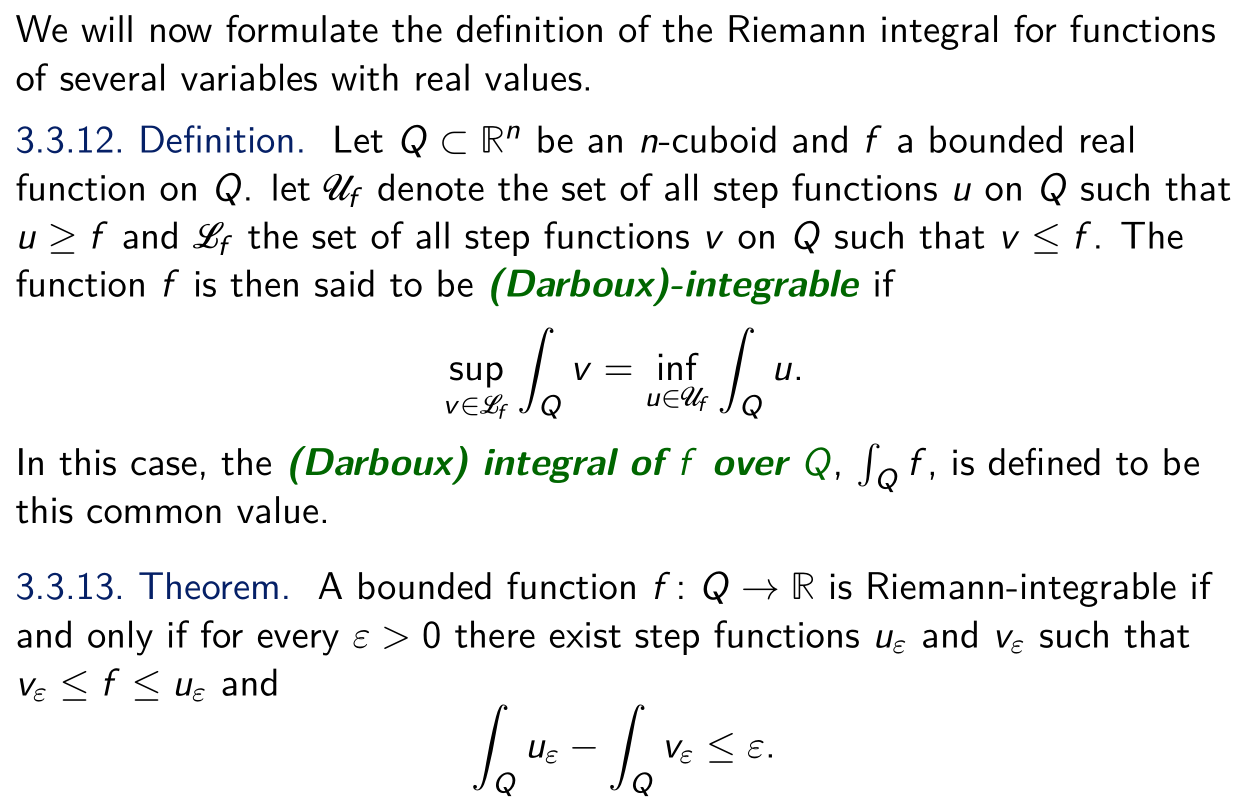
\includegraphics[width=\textwidth]{2020-07-01-11-14-48.png}
    \end{figure}
\end{frame}

\begin{frame}
    \frametitle{Integration over Jordan-Measurable Sets}
    Let $\Omega \subset \mathbb{R}^{n}$ be a bounded Jordan-measurable set and let $f: \Omega \rightarrow \mathbb{R}$ be continuous a.e. Then $f$ is integrable on $\Omega$.
    \nullspace
    That's what we learned in the course. However, we had a hidden precondition here: The function $f$ needs to be bounded on its domain. And in this whole section, we consider only bounded functions. So, to be more precise, the statement should be:
    \nullspace
    Let $\Omega \subset \mathbb{R}^{n}$ be a bounded Jordan-measurable set and let $f: \Omega \rightarrow \mathbb{R}$ be (bounded) and (continuous a.e.). Then $f$ is integrable on $\Omega$.
\end{frame}

\begin{frame}
    \frametitle{Unbounded functions can still be integrable}
    Despite the fact that we only consider bounded functions in this section, we should notice that an unbounded function can still have integrals. (Improper Riemann Integrals)
    \nullspace
    \Question
    $m$ and $n$ are two integers. Judge whether the following integrals exist or not. $\|x\|$ denotes the Euclidean norm.
    \[
        \int_{\mathbb{R}^{n}} \frac{1}{\|x\|^{m}} d x
    \]
    \nullspace
    $(m, n)=(1,2),(1,3),(2,2),(2,3),(3,2),(3,3)$ are the multiple-choice question of final exam in last year! We will talk about this question after learning the substitution rule.

\end{frame}

\subsection{Fubini's Theorem}
\begin{frame}
    \frametitle{Fubini's Theorem}
    Let $Q_1$ be an $n_1$-cuboid and $Q_2$ an $n_2$-cuboid so that $Q:=Q_1\times Q_2\subset\R^{n_1+n_2}$ is an $(n_1+n_2)$-cuboid. Assume that $f:Q\to\R$ is integrable on $Q$ and that for every $x\in Q_1$ the integral
    \[g(x)=\int_{Q_2}f(x,\cdot)\]
    exists. Then
    \[\int_Qf=\int_{Q_1\times Q_2}f=\int_{Q_1}g=\int_{Q_1}\left(\int_{Q_2}f\right).\]

    \Remark This is a very powerful tool. So that we can divide and conquer a integral in $\R^n$.
\end{frame}

\subsection{Ordinate Region}
\begin{frame}
    \frametitle{Ordinate Region}
    For $x\in\R^n$ we define
    \[\hat{x}^{(k)}:=(x_1,\ldots,x_{k-1},x_{k+1},\ldots,
        x_n)\in\R^{n-1}\]
    as the vector $x$ with the $k$th component omitted.\\[4pt]
    A subset $U\subset\R^n$ is said to be an \emph{ordinate region (with respect to $x_k$)} if there exists a measurable set $\Omega\subset\R^{n-1}$ and continuous, almost everywhere dif{}ferentiable functions $\varphi_1,\varphi_2:\Omega\to\R$, such that
    \[U=\{x\in\R^n:x\in\Omega,\varphi_1(\hat{x}^{(k)})\leq
        x_k\leq\varphi_2(\hat{x}^{(k)})\}.\]
    If $U$ is an ordinate region with respect to each $x_k,k=1,\ldots,n$, it is said to be a \emph{simple region}.\\[6pt]
    \Remark Any ordinate region is measurable.
\end{frame}

\begin{frame}
    \frametitle{Exercise}
    Please find the value of following integrals:
    $$\int_{0}^{1} \int_{x}^{1} \sin \left(y^{2}\right) d y d x$$
    $$\int_{0}^{1} \int_{x}^{1} e^{y^{2}} d y d x$$
\end{frame}

\begin{frame}
    \frametitle{Exercise}
    The primitives of $e^{y^{2}}$ and $\sin \left(y^{2}\right)$ are both non-elementary functions, so it's hard for us to integrate them in the original sequence. So we want to change the order of variables. The region can be express by two inequalities:
    \[
        0 \leq x \leq 1, x \leq y \leq 1
    \]
    which is equivalent to
    \[
        0 \leq y \leq 1, \quad 0 \leq x \leq y
    \]
\end{frame}

\begin{frame}
    \frametitle{Exercise}
    Therefore
    \[
        \begin{aligned}
            \int_{0}^{1} \int_{x}^{1} \sin \left(y^{2}\right) d y d x & =\int_{0}^{1} \int_{0}^{y} \sin \left(y^{2}\right) d x d y                            \\
                                                                      & =\int_{0}^{1} y \sin \left(y^{2}\right) d y                                           \\&=               -\left.\frac{\cos \left(y^{2}\right)}{2}\right|_{0} ^{1}\\&=\frac{1-\cos 1}{2}          \\
            \int_{0}^{1} \int_{x}^{1} e^{y^{2}} d y d x               & =\int_{0}^{1} \int_{0}^{y} e^{y^{2}} d x d y                                          \\
                                                                      & =\int_{0}^{1} y e^{y^{2}} d y=\left.\frac{e^{y^{2}}}{2}\right|_{0} ^{1}=\frac{e-1}{2}
        \end{aligned}
    \]


\end{frame}

\subsection{Substitution Rule}
\begin{frame}
    \frametitle{Substitution Rule}
    Here is another powerful tool named substitution rule. Let $\Omega\subset\R^n$ be open and $g:\Omega\to\R^n$ injective and continuously dif{}ferentiable. Suppose that $\det J_g(y)\neq0$ for all $y\in\Omega$. Let $K$ be a compact measurable subset of $\Omega$. The $g(K)$ is compact and measurable and if $f:g(K)\to\R$ is integrable, then
    \[\int_{g(K)}f(x)\,dx=\int_Kf(g(y))\cdot
        \vert\det J_g(y)\vert\,dy.\]
\end{frame}

\begin{frame}[allowframebreaks]
    \frametitle{Applications}
    \begin{enumerate}[(i)]
        \item Polar coordinates in $\R^2$ are defined by a map
              \[\Phi:(0,\infty)\times[0,2\pi)\to\R^2\setminus\{0\},
                  \qquad\quad(r,\phi)\mapsto(x,y)\]
              where
              \[x=r\cos\phi,\qquad\qquad\quad
                  y=r\sin\phi.\]
              Note that this map is bijective and even $C^\infty$ in the interior of its
              domain. An alternative (but rarely used) version of polar coordinates
              would map $x=r\sin\phi,y=r\cos\phi$. This simply corresponds to a
              dif{}ferent geometrical interpretation of the angle $\phi$. In any case,
              \[|\det J_\Phi(r,\phi)|=\left|\det\begin{pmatrix}
                      \cos\phi & -r\sin\phi \\
                      \sin\phi & r\cos\phi
                  \end{pmatrix}\right|=r\]
    \end{enumerate}
    \begin{itemize}
        \item[(ii)] Cylindrical coordinates in $\R^3$ are given through a map
              \[\Phi:(0,\infty)\times[0,2\pi)\times\R\to\R^3\setminus\{0\},\qquad
                  (r,\phi,\zeta)\mapsto(x,y,z)\]
              defined by
              \[x=r\cos\phi,\qquad\quad y=r\sin\phi,\qquad\quad z=\zeta\]
              In this case
              \[|\det J_\Phi(r,\phi,\zeta)|=\left|\det\begin{pmatrix}
                      \cos\phi & -r\sin\phi & 0 \\
                      \sin\phi & r\cos\phi  & 0 \\
                      0        & 0          & 1
                  \end{pmatrix}\right|=r\]

    \end{itemize}
    \newpage
    \begin{spacing}{1.2}
        \begin{itemize}
            \item[(iii)] Spherical coordinates in $\R^3$ are often defined through a map
                  \begin{center}
                      $\Phi:(0,\infty)\times[0,2\pi)\times(0,\pi)\to\R^3\setminus\{0\},\quad
                          (r,\phi,\theta)\mapsto(x,y,z),$\\
                      $x=r\cos\phi\sin\theta,~y=r\sin\phi\sin\theta,~z=r\cos\theta$.
                  \end{center}
                  Of course, there is a certain freedom in defining $\theta$ and $\phi$, so there are
                  alternative formulations. The modulus of the determinant of the
                  Jacobian is given by
                  \begin{equation*}
                      \begin{split}
                          |\det J_\Phi(r,\phi,\theta)| &=\left|\det\begin{pmatrix}
                              \cos\phi\sin\theta & -r\sin\phi\sin\theta & r\cos\phi\cos\theta \\
                              \sin\phi\sin\theta & r\cos\phi\sin\theta  & r\sin\phi\cos\theta \\
                              \cos\theta         & 0                    & -r\sin\theta
                          \end{pmatrix}\right| \\
                          &=r^2\sin\theta
                      \end{split}
                  \end{equation*}
        \end{itemize}
    \end{spacing}
    \newpage
    \begin{itemize}
        \item[(iv)] In $\R^n$, we can define spherical coordinates by
              \begin{align*}
                  x_1     & =r\cos\theta_1                                                   \\
                  x_2     & =r\sin\theta_1\cos\theta_2                                       \\
                  x_3     & =r\sin\theta_1\sin\theta_2\cos\theta_3                           \\
                          & \,\,\,\vdots                                                     \\
                  x_{n-1} & =r\sin\theta_1\sin\theta_2\ldots\sin\theta_{n-2}
                  \cos\theta_{n-1}                                                           \\
                  x_n     & =r\sin\theta_1\sin\theta_2\ldots\sin\theta_{n-2}\sin\theta_{n-1}
              \end{align*}
              with $r>0$ and $0<\theta_k<\pi,k=1,\ldots,n-2,0<\theta_{n-1}<2\pi$. Here,
              \[|\det J_\Phi(r,\theta_1,\ldots,\theta_{n-1})|=r^{n-1}\sin^{n-2}\theta_1
                  \sin^{n-3}\theta_2\ldots\sin\theta_{n-1}.\]
    \end{itemize}
\end{frame}

\begin{frame}
    \frametitle{Exercise}
    The volume of a Jordan-measurable measurable set $\Omega\subset\R^n$ is given by
    \[|\Omega|=\int_\Omega1.\]
    \nullspace
    \Question Calculate the volume of a 4-dimensional unit ball $B^4$.

\end{frame}

\subsection{Improper Integrals}
\begin{frame}
    \frametitle{Improper Integrals}
    Just as for integrals of a single variable, we can treat improper Riemann
    integrals of functions $f:\R^n\to\R$ over measurable sets $\Omega\subset\R^n$. These occur if either
    \begin{enumerate}[1.]
        \item $f$ is unbounded or
        \item $\Omega$ is unbounded.
    \end{enumerate}
    In either case, one considers the improper integral as a suitable limit of
    "proper" integrals; if the limit exists, so does the improper integral.\\[5pt]
\end{frame}

\begin{frame}
    \frametitle{Exercise}
    Now let's review this questions:\\
    $m$ and $n$ are two integers. Judge whether the following integrals exist or not. $\|x\|$ denotes the Euclidean norm.
    \[
        \int_{\mathbb{R}^{n}} \frac{1}{\|x\|^{m}} d x
    \]
    $(m, n)=$
    \begin{enumerate}
        \item (1,2),
        \item (1,3),
        \item (2,2),
        \item (2,3),
        \item (3,2),
        \item (3,3).
    \end{enumerate}
\end{frame}

\begin{frame}
    \frametitle{Exercise}
    With the substitution rule, we can use the spherical coordinates in $\mathbb{R}^{n}$
    \[
        \footnotesize
        \begin{aligned}
            \int_{\mathbb{R}^{n}} \frac{1}{\|x\|^{m}} d x & =\int_{K} \frac{r^{n-1} \sin ^{n-2} \theta_{1} \sin ^{n-3} \theta_{2} \ldots \sin \theta_{n-1}}{r^{m}} d r d \theta_{1} d \theta_{2} \cdots d \theta_{n-1}                      \\
                                                          & =\left(\int_{0}^{\pi} \sin ^{n-2} \theta_{1} d \theta_{1}\right) \cdots\left(\int_{0}^{\pi} \sin \theta_{n-1} d \theta_{n-1}\right)\left(\int_{0}^{\infty} r^{n-m-1} d r\right)
        \end{aligned}
    \]
    We can just consider whether $\int_{0}^{\infty} r^{n-m-1} d r$ exists For all $k \in \mathbb{Z},$ the targeted value of $\int_{0}^{\infty} r^{k} d r$ is $\infty,$ so all of the integrals do not exist.
\end{frame}

\begin{frame}
    \frametitle{Exercise}
    What if we replace $\R^n$ by $B^n$?
    \nullspace
    If the integral $$\int_{B^n} \frac{1}{\|x\|^{m}} d x$$ in $\mathbb{R}^{n}$ exists, what relationship does $n$ and $m$ have?
    \nullspace
    \pause $(n \geq m+1)$
\end{frame}

\subsection{Parametrized Surface}
\begin{frame}
    \frametitle{Parametrized Surface}
    A \emph{smooth parametrized m-surface in $\R^n$} is a subset $\mathcal{S}\subset\R^n$ together with a locally bijective, continuously dif{}ferentiable map (parametrization)
    \[\varphi:\Omega\to\mathcal{S},\qquad\quad
        \Omega\subset\R^m,\]
    such that
    \[\text{rank}\,D\varphi|_x=m\]
    for almost every $x\in\Omega$. If $m=n-1$, $\mathcal{S}$ is said to be a \emph{parametrized hypersurface}.
\end{frame}

\subsection{Tangent Spaces of Surface}
\begin{frame}
    \frametitle{Tangent Spaces of Surface}
    Let $\mathcal{S}\subset\R^n$ be a parametrized $m$-surface with parametrization $\varphi:\Omega\to\mathcal{S}$. Then
    \[t_k(p)=\frac{\partial}{\partial x_k}\left.\begin{pmatrix}
            \varphi_1(x) \\
            \vdots       \\
            \varphi_n(x)
        \end{pmatrix}\right|_{x=\varphi^{-1}(p)},\qquad\quad
        k=1,\ldots,m.\]
    is called the \emph{$k$th tangent vector of $\mathcal{S}$ at $p\in\mathcal{S}$} and
    \[T_p\mathcal{S}:=\text{ran}\,D\varphi|_x
        =\text{span}\{t_1(p),\ldots,t_m(p)\}\]
    is called the \emph{tangent space} to $\mathcal{S}$ at $p$. The vector field
    \[t_k:\mathcal{S}\to\R^n,\qquad\qquad\quad
        p\mapsto t_k(p)\]
    is called the \emph{$k$th tangent vector field} on $\mathcal{S}$.
\end{frame}

\begin{frame}
    \frametitle{Exercise}
    $\operatorname{Let} S^{2}=\left\{(x, y, z) \in \mathbb{R}^{3}: x^{2}+y^{2}+z^{2}=1\right\}$ be the unit sphere and $p=(a, b, c) \in S^{2} .$ Show that the tangent plane at $p$ is given by
    \[
        T_{p} S^{2}=\left\{(x, y, z) \in \mathbb{R}^{3}: a x+b y+c z=1\right\}
    \]
\end{frame}

\begin{frame}[allowframebreaks]
    \frametitle{Solution 1}
    We parametrize the unit sphere by
    \[
        \Phi(\phi, \theta)=\left(\begin{array}{c}
                \cos \phi \sin \theta \\
                \sin \phi \sin \theta \\
                \cos \theta
            \end{array}\right)
    \]
    The tangent vectors at the point $p$ are
    \[
        \begin{array}{l}
            t_{\phi}(p)=\left.\frac{\partial}{\partial \phi}\left(\begin{array}{c}
                    \cos \phi \sin \theta \\
                    \sin \phi \sin \theta \\
                    \cos \theta
                \end{array}\right)\right|_{p}=\left.\left(\begin{array}{c}
                    -\sin \phi \sin \theta \\
                    \cos \phi \sin \theta  \\
                    0
                \end{array}\right)\right|_{p} \\
            t_{\theta}(p)=\left.\frac{\partial}{\partial \theta}\left(\begin{array}{c}
                    \cos \phi \sin \theta \\
                    \sin \phi \sin \theta \\
                    \cos \theta
                \end{array}\right)\right|_{p}=\left.\left(\begin{array}{c}
                    \cos \phi \cos \theta \\
                    \sin \phi \cos \theta \\
                    -\sin \theta
                \end{array}\right)\right|_{p}
        \end{array}
    \]
    The point $q=(x, y, z) \in T_{p} S^{2}$ if and only if $q-p \in \operatorname{span}\left\{t_{\phi}(p), t_{\theta}(p)\right\},$ so
    \[
        \left.\operatorname{det}\left(\begin{array}{ccc}
                x-a & -\sin \phi \sin \theta & \cos \phi \cos \theta \\
                y-b & \cos \phi \sin \theta  & \sin \phi \cos \theta \\
                z-c & 0                      & -\sin \theta
            \end{array}\right)\right|_{p}=0
    \]
    Evaluating the determinant, we obtain
    \[
        \footnotesize
        (x-a)\left(-\sin ^{2} \theta \cos \phi\right)+(y-b)\left(-\sin ^{2} \theta \sin \phi\right)+(z-c)(-\sin \theta \cos \theta)=0
    \]
    Dividing by $\sin \theta$ and inserting the parametrization, we obtain
    \[
        (x-a) x+(y-b) y+(z-c) z=0
    \]

    Using $x^2 + y^2 + z^2 = 1$, we obtain $ax + by + cz = 1$.
\end{frame}

\begin{frame}
    \frametitle{Solution 2}
    It is known that the tangent vectors to the sphere at $p$ are orthogonal to $p,$ so $q \in T_{p} S^{2}$ if and only if $\langle q-p, p\rangle=0 .$ This is equivalent to
    \[
        \langle q, p\rangle=\langle p, p\rangle=1
    \]
    which also gives $a x+b y+c z=1$


\end{frame}

\subsection{Normal Vector to Hypersurface}
\begin{frame}
    \frametitle{Normal Vector to Hypersurface}
    Let $\mathcal{S}\subset\R^n$ be a hypersurface. Then a unit vector that is orthogonal to all tangent vectors to $\mathcal{S}$ at $p$ is called a \emph{unit normal vector to $\mathcal{S}$ at $p$} and denoted by $N(p)$. The vector field
    \[N:\mathcal{S}\to\R^n,\qquad\qquad\quad
        p\mapsto N(p)\]
    is called the \emph{normal vector field} on $\mathcal{S}$.

    \begin{enumerate}[(i)]
        \item A hypersurface that is the boundary of a measurable set $\Omega\subset\R^n$ with non-zero measure is said to be a \emph{closed surface}.
        \item A closed hypersurface is said to have \emph{positive orientation} if the
              normal vector field is chosen so that the normal vectors point
              outwards from $\Omega$. (Important. We will discuss flux and divergence of a vector field later.)
    \end{enumerate}
\end{frame}

\begin{frame}
    \frametitle{Area of Hypersurface}

    We define the \emph{scalar surface element of a hypersurface in $\R^3$} by
    \[dA=|\det(t_1,t_2,N)\circ\varphi|dx_1\,dx_2.\]
    Of course, we can generalize this to hypersurfaces in $\R^n$, setting
    \[dA=|\det(t_1,t_2,\ldots,t_{n-1},N)\circ
        \varphi|\,dx_1\,dx_2\ldots dx_{n-1}.\]

    We can then define the area of a hypersurface:
    The \emph{volume} or \emph{area} of $\mathcal{S}$ is defined as
    \[|\mathcal{S}|:=\int_\Omega|\det(t_1,\ldots,t_{n-1},N)
        \circ\varphi(x)|\,dx_1\,dx_2\ldots dx_{n-1}.\]

    \Remark We define the $dA$ in this way because we have not developed a way to directly represent it without recourse to $N$. However, with the help of \emph{metric tensor}, we can.
\end{frame}

\begin{frame}
    \frametitle{Metric Tensor}
    Let $\mathcal{S}\subset\R^n$ be an $m$-surface with parametrization $\varphi$ and tangent vector fields \myseries{t}{m}. Then $G\in\text{Mat}(m\times m;\R)$ given by
    \[G:=\begin{pmatrix}
            \scp{t_1}{t_1} & \cdots & \scp{t_1}{t_m} \\
            \vdots         & \ddots & \vdots         \\
            \scp{t_m}{t_1} & \cdots & \scp{t_m}{t_m}
        \end{pmatrix}\]
    is said to be the \emph{metric tensor} on $\mathcal{S}$ with respect to $\varphi$.
    \nullspace
    \Remark By the definition of metric tensor, we immediately have
    $$\left|\operatorname{det}\left(t_{1}, \ldots, t_{n-1}, N\right)\right|=\sqrt{\operatorname{det} G}$$
    The significance of metric tensor is: we don't bother ourselves to calculate the normal vector if we want to find $dA$.
\end{frame}

\begin{frame}
    \frametitle{$dA$ in $\R^3$}
    The scalar surface element in $\R^3$ has two equivalent forms:
    \begin{enumerate}
        \item \[dA=|\det(t_1,t_2,N)\circ\varphi|dx_1\,dx_2.\]
        \item $$d A=\left\|t_{1} \times t_{2}\right\| \circ \varphi(x) d x_{1} d x_{2}$$
    \end{enumerate}
    \nullspace
    \Remark Calculation in $\R^3$ is sometimes tedious. You might want to use \textit{Mathematica} to help you find the solution. It is quite feasible, even during the exam. However, you need to show all your necessary procedures in your solutions. We will be very strict in grading your procedures in Mid2.
\end{frame}

\subsection{Scalar Surface Integrals}
\begin{frame}
    \frametitle{Scalar Surface Integrals}
    Let $\mathcal{S}$ be a parametrized $m$-surface with parametrization $\varphi:\Omega\to\mathcal{S},\Omega\subset\R^m$. Then
    \[|\mathcal{S}|:=\int_\Omega\sqrt{g(x)}dx\]
    defines the \emph{volume} or \emph{area} of $\mathcal{S}$.\\[4pt]
    Let $f:\mathcal{S}\to\R$ be a potential function. Then the \emph{(scalar) surface integral of $f$ over $\mathcal{S}$} is defined as
    \[\int_\mathcal{S}f\,dA:=\int_\Omega f\circ\varphi(x)\sqrt{g(x)}\,dx\]
    \Remark As usual,
    \[dA:=\sqrt{g(x)}\,dx\]
    is called the \emph{scalar surface element} of $\mathcal{S}$.
\end{frame}

\begin{frame}
    \frametitle{Remark}
    In practice. the calculus is tedious. Here are the general steps of solving a scalar surface integral problem.

    \begin{enumerate}
        \item Clarify the parametrization of the surface. (You might choose convenient coordinates in this step.)
        \item Find the tangent vectors of the surface.
        \item Use the metric tensor or normal vector to find $dA$.
        \item Perform the scalar surface integral.
    \end{enumerate}

    You can directly give the volume/area of some regular objects in the exam without rigorous proof, e.g. sphere, cube, cylinder.
\end{frame}

\begin{frame}
    \frametitle{Important Summary}
    Make sure you prepare well before the exam. i.e. You know how to perform any of these integrals \textbf{in details}. I did not prepare enough examples for all kinds of integrals we learned due to time limitation. But to better prepared yourself for the exam (and future study), I strongly recommend you to find some exercises that are ugly and tedious enough and solve them by yourself. (Ugly and tedious: There is no symmetry/The region is not a cuboid/The result is not 0/You may need to use substitution rule and Fubini's theorem.)
    \nullspace
    Here is a website that might help: \href{https://tutorial.math.lamar.edu/problems/calciii/SurfaceIntegralsIntro.aspx}{Paul's Online Notes}.
    \nullspace
    In addition, we will look at some interesting examples regarding area/volume integrals on Friday (discussion class hosted by TA Wang Ruiyi).

\end{frame}


\begin{frame}
    \frametitle{About Assignment 8}
    Particularly pay attention to these problems:
    \begin{itemize}
        \item[8.1] Calculate area of given surfaces.
        \item[8.2] Calculate surface integrals (on scalar function).
        \item[8.4] Calculate line integrals (on scalar function).
    \end{itemize}

    They are all good practices for you (to get familiar with integrals).
\end{frame}



\begin{frame}
    \frametitle{Discussion}
    \vspace{1cm}
    \begin{center}
        \LARGE
        Have Fun\\
        And\\
        Learn Well!
    \end{center}
    \vspace{2cm}
    \footnotesize Acknowledgement: I would like to express my gratitude to TA Jin Haoxiang. Many examples in my RC are provided by him.
\end{frame}

\end{document}